\documentclass[a4paper]{article}
\usepackage{latexsym}
\usepackage[a4paper]{geometry}
\usepackage{color}
\usepackage{listings}
\usepackage[pdftex]{graphicx}
\usepackage{subfig}
\usepackage{float}

\definecolor{Blue}{rgb}{0,0,0.5}
\definecolor{Green}{rgb}{0,0.75,0.0}
\definecolor{LightGray}{rgb}{0.6,0.6,0.6}
\definecolor{DarkGray}{rgb}{0.3,0.3,0.3}
\lstset{language=Matlab,
   keywords={function,uint8,uint16,uint32,double,break,case,catch,continue,else,elseif,end,for,global,if,otherwise,persistent,return,switch,try,while},
   basicstyle=\ttfamily\small,
   breaklines=true,
   keywordstyle=\bfseries\color{Blue},
   commentstyle=\itshape\color{LightGray},
   stringstyle=\color{Green},
   numbers=left,
   numberstyle=\tiny\color{DarkGray},
   stepnumber=1,
   numbersep=10pt,
   backgroundcolor=\color{white},
   tabsize=2,
   showspaces=false,
   showstringspaces=false,
   captionpos=b}

%Boldface text for type writer font
\usepackage{bold-extra} %\DeclareFontShape{OT1}{cmtt}{bx}{n}{<5><6><7><8><9><10><10.95><12><14.4><17.28><20.74><24.88>cmttb10}{}

%Break words properly at the end of a line (which isn't sloppy...)
\sloppy

%Use command \exercise for each exercise
\newcounter{exerciseCount}
\setcounter{exerciseCount}{0}
\newcommand{\exercise}[1]{\addtocounter{exerciseCount}{1} \noindent \medskip {\large \textsf{\textbf{Exercise \arabic{exerciseCount} \--- #1}}} \par}
\renewcommand{\theenumi}{\textsf{\textbf{\alph{enumi}}}}

%Use command \code for code snippets
\newcommand{\code}[1]{\textnormal{\texttt{#1}}}



\title{\textsf{Image Processing \\ lab 2}}
\author{Klaas Kliffen \and Jan Kramer}
\date{\today}

\begin{document}
\maketitle

\exercise{Fourier spectrum}
\begin{enumerate}
\item
% TODO: explain the code
The functions build in functions fft2 and fftshift are used to create the fourier spectrum 
image centered around the DC component of the fourier transform.
Some extra code is added for calculating the average of the image, which will be explained in more
detail in part c of this exercise.
To be able to view the spectrum, the values need to be scaled. So the log is taken of each value
to increase the constrast.
\lstinputlisting{../lab2ex1/runex1.m}
\item 
\begin{figure}[H]
\centering

\includegraphics[width=.5\textwidth]{../lab2ex1/characters.png}
\caption{Original image}
\label{fig:chars}
\end{figure}
\begin{figure}[H]
\centering
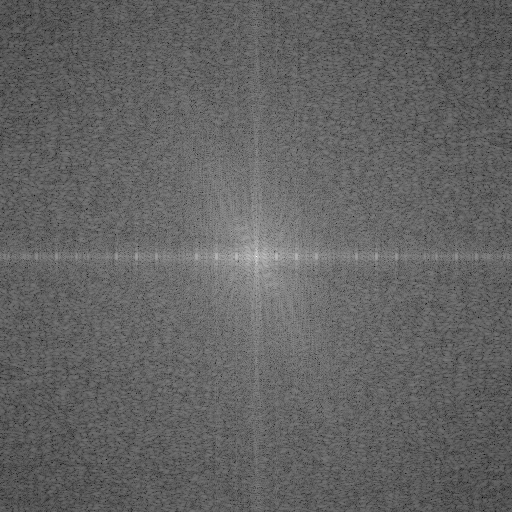
\includegraphics[width=.5\textwidth]{../lab2ex1/spectrum.png}
\caption{Fourier spectrum of figure \ref{fig:chars}}
\end{figure}
\item
% TODO: explain why the DC factor div numpixs = average
The maginitude of the center of the image is the DC component.
For images, this is the sum of the grey levels of all pixels.
Dividing this by the number of pixels gives the average grey level.
In this case:  207.31 for figure \ref{fig:chars}.
This value is equal to the result achieved by using \lstinline|mean| two times.
\end{enumerate}

\newpage

\exercise{Highpass filtering in the frequency domain}
\begin{enumerate}
\item 
The Gaussian highpass transfer function is given by
\begin{displaymath}
H(u,v) = 1 - e^{- \frac{{D(u,v)}^2}{2 \cdot D_{0}^2}} = 1 - e^{- \frac{(u - P/2)^2 + (v - Q/2)^2}{2 \cdot D_{0}^2}}
\end{displaymath}
where $P \geq 2\cdot M - 1$, $ Q \geq 2 \cdot N - 1$, $u = [0, P-1]$ and $v = [0, Q-1]$.
This function is used to lessen the strength of low frequencies in a spectrum by multiplying it elementwise with said spectrum.
An example can be seen in Figure~\ref{fig:ghpf}.
Note that the white part allow the frequencies to pass through, while the black part weakens low frequencies if the spectrum is centered.
\begin{figure}[H]
\centering

\includegraphics[width=.5\textwidth]{../lab2ex2/filter.png}
\caption{The Gaussian highpass filter with $D_{0} = 30$}
\label{fig:ghpf}
\end{figure}
Another thing to note is that filter size is bigger than the image size.
The reason for this is that the image is expected to be padded to prevent wraparound errors as shown in Figure~4.32 in the book.
%TODO: explain the code
\lstinputlisting{../lab2ex2/IPgaussian.m}
\item
The general way of applying filters in the frequency domain is summarized in Section 4.7.3 of the book.
In the case of IPftfilter the steps are as follows:
\begin{description}
\item[Step 1] Pad the image to the size of the filter to prevent wraparound errors.
\item[Step 2] Perform DFT on this padded image to get the spectrum.
\item[Step 3] Apply the given filter to the spectrum.
\item[Step 4] Perform the inverse DFT on the new spectrum and take the real parts.
\item[Step 5] Extract the final image by removing the padding.
\end{description}
Note that this can also be done with every spectrum shifted to the center.
This does not influence the result, so it was omited.
%TODO: explain the code
\lstinputlisting{../lab2ex2/IPftfilter.m}
\item
\begin{figure}[H]
\centering
\begin{tabular}{cc}
    
\includegraphics[width=0.4\textwidth]{../lab2ex1/characters.png} &
    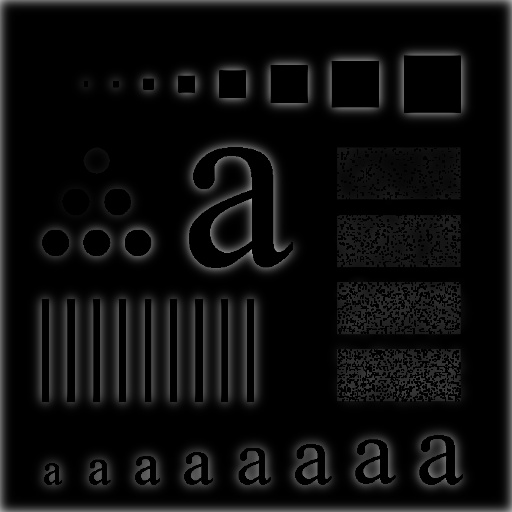
\includegraphics[width=0.4\textwidth]{../lab2ex2/characters-GHPF-D30.png} \\
    Original image & $D_{0} = 30$ \\
    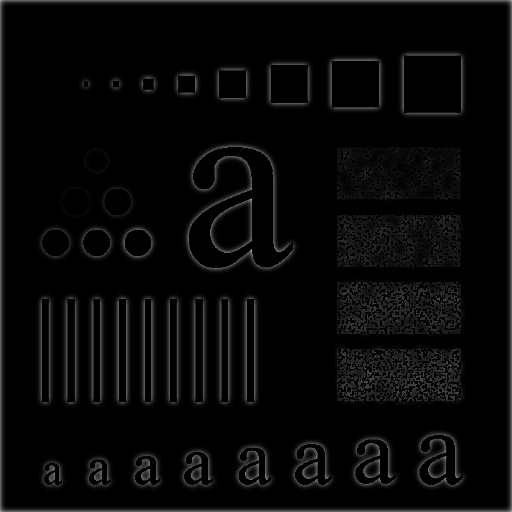
\includegraphics[width=0.4\textwidth]{../lab2ex2/characters-GHPF-D60.png} &
    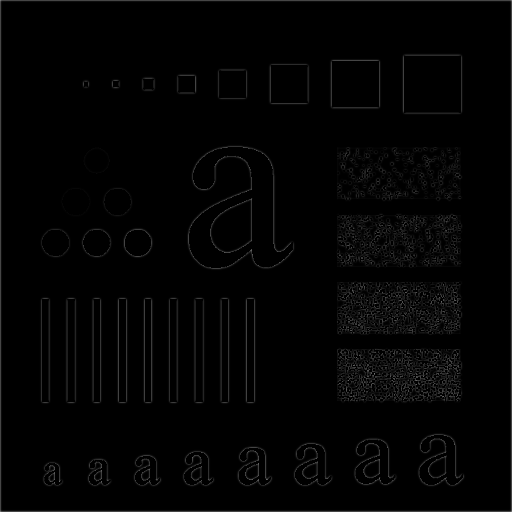
\includegraphics[width=0.4\textwidth]{../lab2ex2/characters-GHPF-D160.png} \\
    $D_{0} = 60$ & $D_{0} = 160$ \\
\end{tabular}
\caption{Gausian Highpass Filtering}
\end{figure}
\end{enumerate}

\exercise{Median filtering}
\begin{enumerate}
\item
%TODO: explain the code
The \lstinline|IPmedian| function takes the distorted image and a value k as its input parameters.
The for each pixel in the image, a window is created with width and height of $2k+2$.
When encountering a boundary, the windowsize is decreased to fit the image.
A submatrix is then used to represent all the pixels in the window.
From this submatrix, the median is calculated and used for the output image.
\lstinputlisting{../lab2ex3/IPmedian.m}
\item
\begin{figure}[H]
\centering
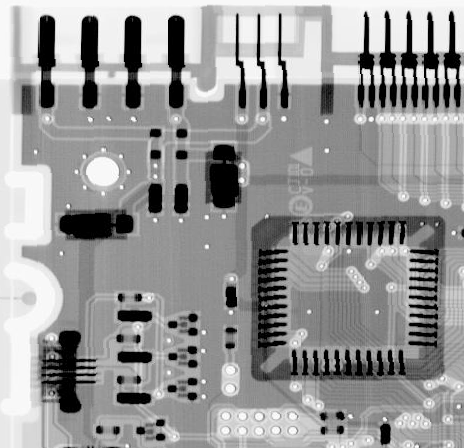
\includegraphics[width=.5\textwidth]{../lab2ex3/circuitboard.png}
\caption{Original image of the circuitboard}
\label{fig:circuit}
\end{figure}
\begin{figure}[H]
\centering
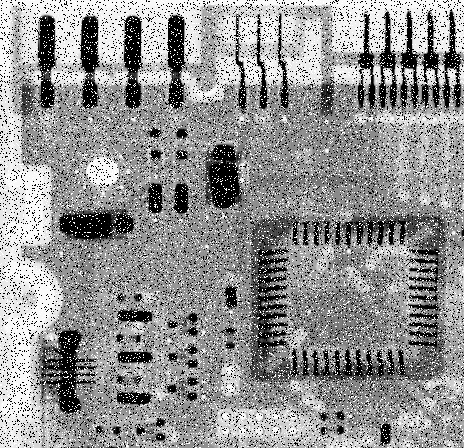
\includegraphics[width=.5\textwidth]{../lab2ex3/noise.png}
\caption{Figure \ref{fig:circuit} with salt \& pepper noise with $Pa = Pb = 0.2$}
\label{fig:noise}
\end{figure}
\item
%TODO: place all the images
\begin{figure}[H]
\centering
\begin{tabular}{cc}
    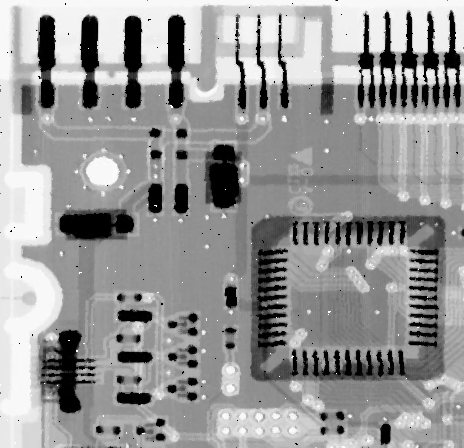
\includegraphics[width=0.4\textwidth]{../lab2ex3/restored1.png} &
    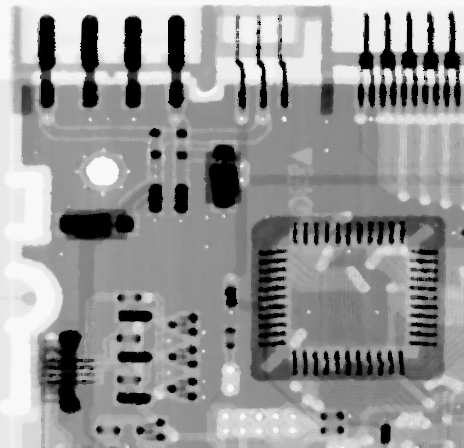
\includegraphics[width=0.4\textwidth]{../lab2ex3/restored2.png}\\
    $k = 1$ & $k = 2$ \\
    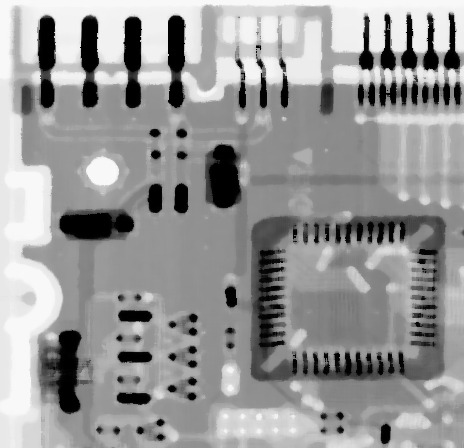
\includegraphics[width=0.4\textwidth]{../lab2ex3/restored3.png} &
    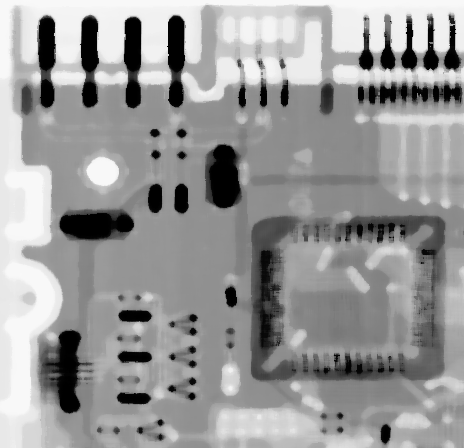
\includegraphics[width=0.4\textwidth]{../lab2ex3/restored4.png}\\
    $k = 3$ & $k = 4$
    
\end{tabular}
\caption{Using median filtering with different window values $k$ on figure \ref{fig:noise}} 
\label{fig:restored}
\end{figure}
In the image created by filtering with $k=1$, some noise is still present.
This is equal to the image 5.10b in the book. Using $k=2$ removes all noise particles.
Increasing k further reduces the sharpness of the image as can be seen in the two lower 
images in \ref{fig:restored}
\end{enumerate}

\newpage
\section*{Task distribution}

\begin{table}[H]
\centering
\begin{tabular}{ccccc}
ex1 & design & implementation & answers questions & writing report \\
\hline
Klaas & 50\% & 100\% & 50\% & 50\% \\
\hline
Jan & 50\% & 0\% & 50\% & 50\% \\
\end{tabular}
\end{table}

\begin{table}[H]
\centering
\begin{tabular}{ccccc}
ex2 & design & implementation & answers questions & writing report \\
\hline
Klaas & 50\% & 0\% & 50\% & 50\% \\
\hline
Jan & 50\% & 100\% & 50\% & 50\% \\
\end{tabular}
\end{table}

\begin{table}[H]
\centering
\begin{tabular}{ccccc}
ex3 & design & implementation & answers questions & writing report \\
\hline
Klaas & 50\% & 100\% & 50\% & 50\% \\
\hline
Jan & 50\% & 0\% & 50\% & 50\% \\
\end{tabular}
\end{table} 



\end{document}
